\chapter{Evaluation of Results}

This is another chapter that I consider particularly important. So far, so good — training, synthesis, and generation of synthetic data for various analytical purposes have been presented, but how can I know how efficiently the work has been carried out?  
How can I assess whether the model is truly capable of contributing effectively in contexts where we genuinely need to generate reliable data?  
Fortunately, there are a number of quantitative measures that provide concrete support for this verification.  
It is therefore useful to give an overview of the metrics I adopted, how I measured the performances, how I compared real and synthetic data, to discuss the limitations observed, and finally to reflect on the results in relation to the initial project objectives.  
Clearly, all this is essential to obtain meaningful feedback on the effectiveness of the work performed.

\section{Metrics Adopted}

To measure the numerical and structural fidelity of the synthetic generations, I adopted a set of metrics commonly used in the literature on multivariate time series~\cite{hyndman2006another,willmott2005advantages,han2011data}.  
The main ones are listed below:

\[
\mathrm{MAE} = \frac{1}{n}\sum_{i=1}^{n} |y_i - \widehat{y}_i|, 
\quad
\mathrm{RMSE} = \sqrt{\frac{1}{n}\sum_{i=1}^{n}(y_i - \widehat{y}_i)^2},
\]
\[
\mathrm{sMAPE} = \frac{100}{n}\sum_{i=1}^{n}
\frac{2\,|\,\widehat{y}_i - y_i\,|}{|\,\widehat{y}_i\,| + |\,y_i\,| + \varepsilon},
\quad
\mathrm{Corr} = \mathrm{corr}_{\text{Pearson}}(y, \widehat{y}).
\]

\begin{itemize}
  \item \textbf{MAE (Mean Absolute Error)} — measures the average absolute difference between real and estimated values, providing a direct indication of model accuracy in the same units as the analyzed variable.
  
  \item \textbf{RMSE (Root Mean Square Error)} — penalizes large deviations more strongly than MAE, making it particularly useful for identifying outliers or local anomalies.
  
  \item \textbf{sMAPE (Symmetric Mean Absolute Percentage Error)} — expresses the relative error as a percentage, normalized with respect to the amplitude of real and synthetic values. Its symmetry prevents distortions in cases of large-scale variability.
  
  \item \textbf{Pearson correlation} — evaluates the linear consistency between two time series, assuming values between $-1$ and $1$. Unlike error metrics, it quantifies the model’s ability to reproduce the trend and overall shape of the signal over time.
\end{itemize}

All evaluations were performed on the HPC datasets considered in the project, applying the three conditional generation masks \emph{F, C, M}.  
The real and synthetic series were aligned using \texttt{merge\_asof} on timestamps, which, as recalled earlier, ensures consistent comparison even in the presence of slight temporal discrepancies.

\paragraph{Implementation.}
The following code shows in compact form the functions used for calculating the basic evaluation metrics.  
All functions return scalar values that can be easily compared across datasets and configurations.

\begin{listing}[H]
\begin{minted}[fontsize=\footnotesize,breaklines,linenos,frame=lines,bgcolor=lightgray!10]{python}
import numpy as np

def mae(y, yhat):
    return float(np.mean(np.abs(np.asarray(yhat) - np.asarray(y))))

def rmse(y, yhat):
    return float(np.sqrt(np.mean((np.asarray(yhat) - np.asarray(y))**2)))

def smape(y, yhat, eps=1e-8):
    y, yhat = np.asarray(y), np.asarray(yhat)
    return float(np.mean(2 * np.abs(yhat - y) /
                         (np.abs(yhat) + np.abs(y) + eps)) * 100)

def pearson_corr(y, yhat):
    y, yhat = np.asarray(y), np.asarray(yhat)
    if y.size < 2 or np.std(y) == 0 or np.std(yhat) == 0:
        return float("nan")
    return float(np.corrcoef(y, yhat)[0, 1])
\end{minted}
\caption{Compact implementation of basic evaluation metrics.}
\end{listing}

\paragraph{Evaluation Scenarios.}
I applied the metrics described above in two distinct yet complementary scenarios, in order to evaluate the model’s behavior both in the presence of real reference data and in purely generative contexts:

\begin{enumerate}
  \item \emph{Forecast with available ground truth} — in this scenario, the real future series is known and used as a direct reference. The comparison between actual and predicted values makes it possible to assess both predictive accuracy and the model’s ability to generalize to unseen data.
  
  \item \emph{Tail proxy} — when future observations are not available, the evaluation relies on the comparison between the latest real windows and the corresponding synthetic sequences generated by the model. This provides a surrogate indicator of predictive consistency and dynamic stability.
\end{enumerate}

This dual approach ensures a balance between \textbf{numerical rigor} and \textbf{methodological flexibility}, allowing me to analyze performance consistently in both explicit forecasting and fully generative scenarios.


\section{Comparison between Real and Synthetic Data}

I then conducted an initial series of experiments on the \emph{M2M} dataset, selecting \texttt{3Phase System Active Power AVG} as the reference variable.

\paragraph{Methodology.}
For each evaluation scenario, I compared the synthetic sequences produced with their corresponding real segments — in the case of forecasts with available ground truth — or with their respective tails, when future observations were unknown (\emph{tail proxy}).  
The metrics adopted, consistent with the framework defined by the authors of \emph{WaveStitch}, include:
\begin{itemize}
  \item the \textbf{mean square error (MSE)}, used to measure numerical accuracy;
  \item the \textbf{autocorrelation difference (ACD)}, used to evaluate the fidelity of internal temporal dynamics;
  \item the \textbf{cross-correlation difference (x-CorrDiff)}, used to quantify the preservation of multivariate relationships between correlated variables.
\end{itemize}
This approach allowed me to analyze both the point accuracy of forecasts and the statistical consistency of the generated patterns over time in a balanced way.

\paragraph{Results on \emph{M2M}.}
With regard to the aggregated \emph{M2M} dataset, I observed an almost perfect alignment between real and synthetic series: seasonal fluctuations are reproduced with high precision, and the model manages to capture both the global periodicity and the local structure of the signal.  
The MSE values are low, and the structural indices \textbf{ACD} and \textbf{x-CorrDiff} confirm the internal consistency of the generated signal.  
In numerical terms, the average differences in autocorrelation and cross-correlation remain at very low levels, indicating that the model faithfully preserves the underlying temporal and multivariate relationships.

\paragraph{Extension to Individual Racks.}
I then replicated the analysis on the individual rack datasets (\emph{RackNpduA}), characterized by more discontinuous and noisy signals.  
In the absence of future data, the evaluation was based on a comparison of real and synthetic tails.  
In this more complex context, the model maintained good stability and continuity, showing only a marginal increase in errors — consistent with the impulsive nature of local signals.

\begin{table}[H]
\centering
\caption{Structural fidelity between real and synthetic series (mean values on tail $N{=}5000$, z-score). Lower values indicate greater temporal and multivariate consistency.}
\vspace{1mm}
{\small
\begin{tabular}{| l | c | c | c | c |}
\hline
\rowcolor[HTML]{F87C58}
\textbf{Dataset} & \textbf{Mask} & \textbf{n\_features} & \textbf{ACD\_mean} & \textbf{xCorrDiff\_mean} \\
\hline
\rowcolor[HTML]{FDE5DC}
M2M       & F/C/M & 9  & 0.130 & 0.358 \\ \hline
\rowcolor[HTML]{FFF4EE}
Rack2pduA & F/C/M & 16 & 0.699 & 0.491 \\ \hline
\end{tabular}
}
\label{tab:acd_xcorr_summary_1}
\end{table}

\paragraph{Visualization.}
To verify this visually, I compared the real and synthetic segments of the series, observing the perfect continuity of transitions between overlapping windows.  
In the \emph{M2M} dataset, the model preserves oscillations and seasonality in a natural way; in the individual racks, on the other hand, more irregular fluctuations emerge due to the impulsive nature of the signals, yet the average trend remains consistent.

\begin{figure}[H]
\centering
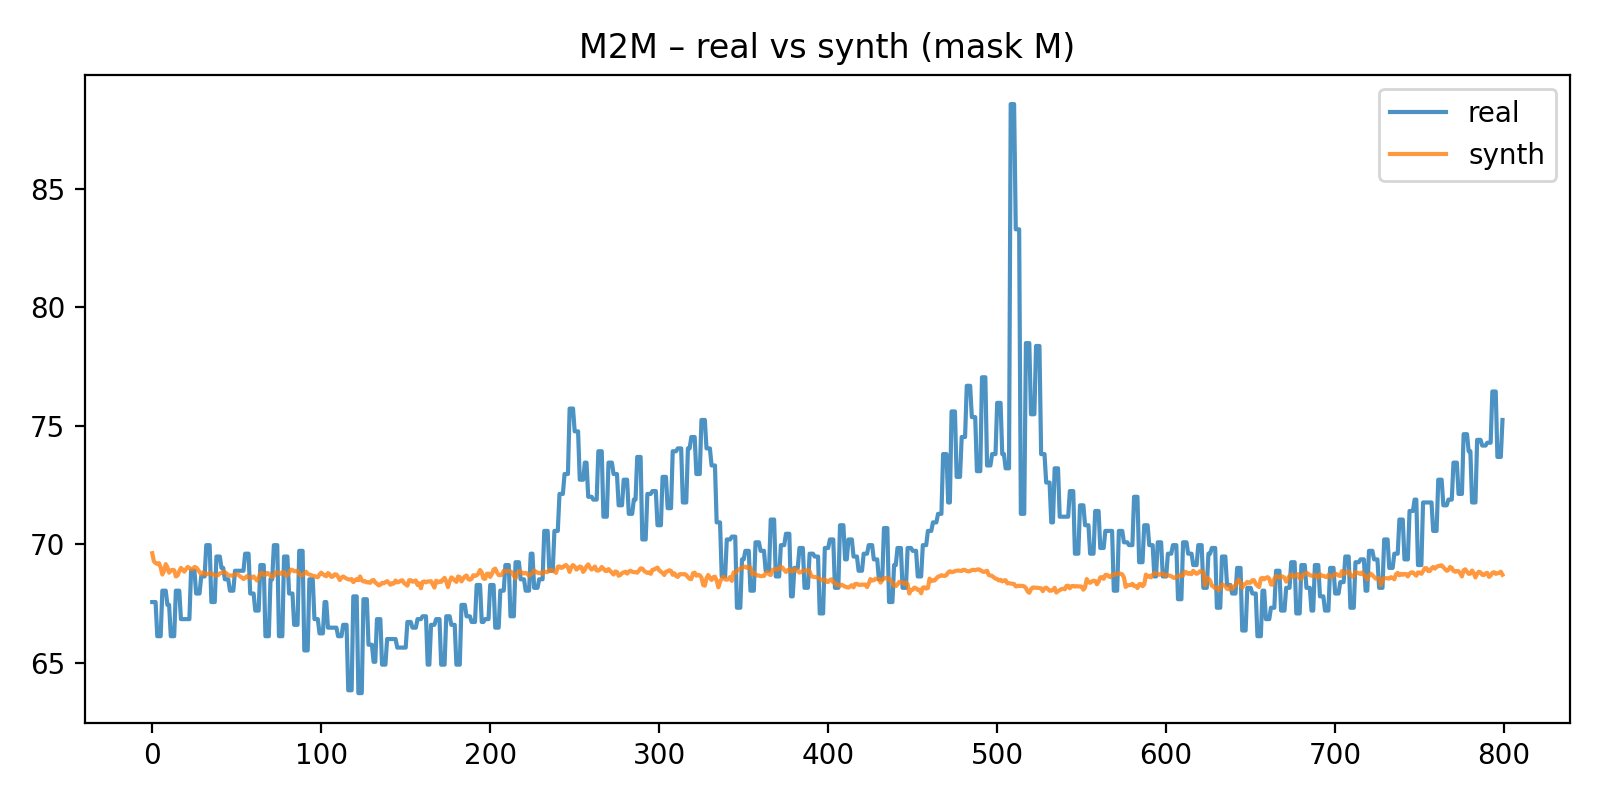
\includegraphics[width=0.85\textwidth]{images/M2M_stitch_real_synth.png}
\caption{Comparison between real and synthetic sequences on \emph{M2M}: the model maintains periodicity and structural continuity.}
\label{fig:m2m_stitch_real_synth}
\end{figure}

\begin{figure}[H]
\centering
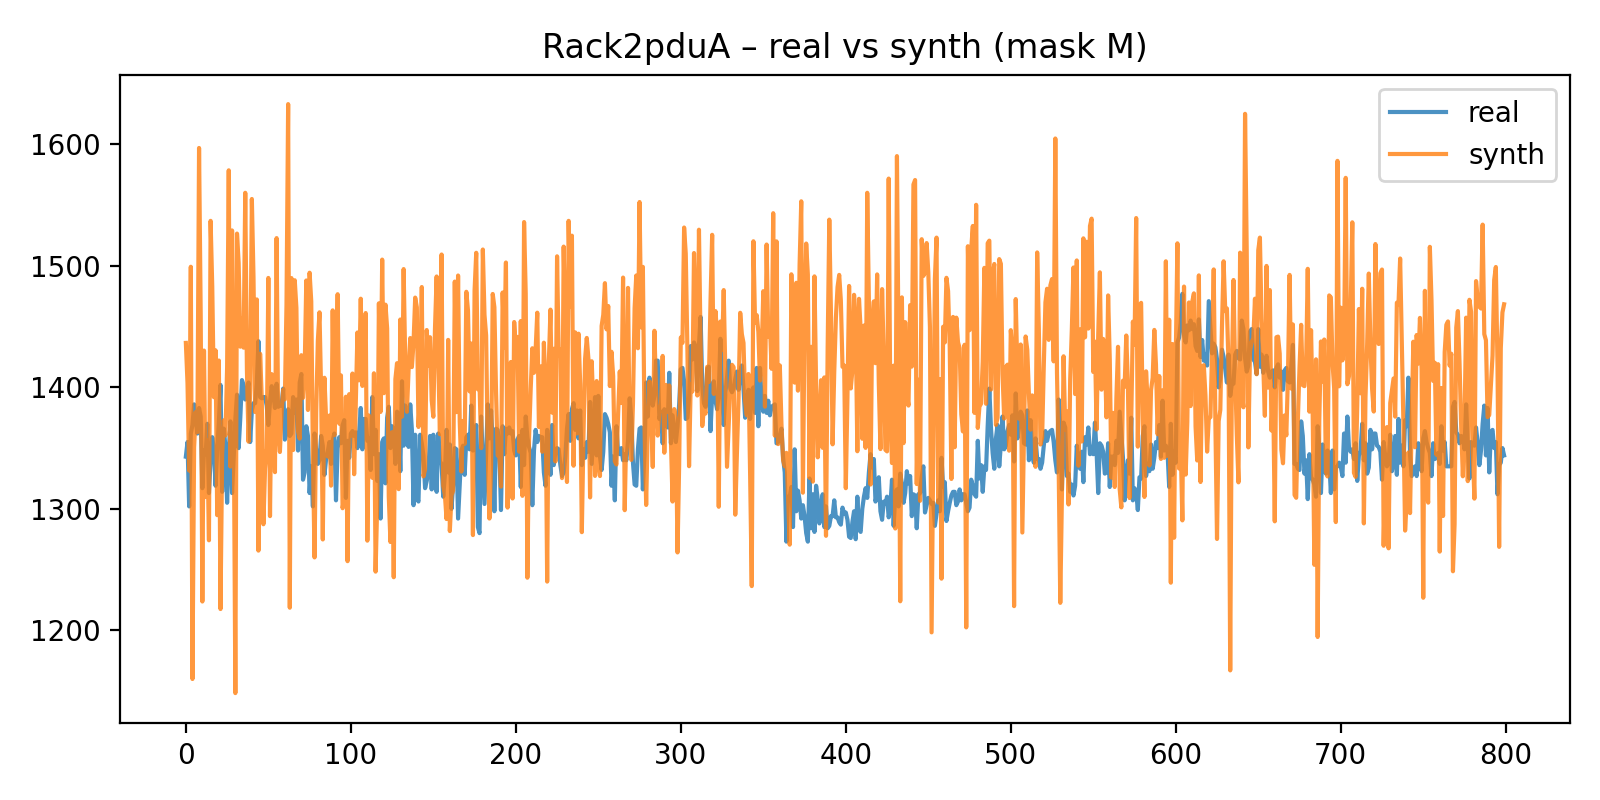
\includegraphics[width=0.85\textwidth]{images/Rack2pduA_stitch_real_synth.png}
\caption{Real–synthetic comparison on \emph{Rack2pduA}: greater variability and noise, but statistical consistency preserved.}
\label{fig:rack2pdua_stitch_real_synth}
\end{figure}

\paragraph{Discussion.}
The results obtained demonstrate that \emph{WaveStitch} is capable not only of accurately reproducing numerical values (low MSE), but also of preserving the temporal and multivariate dependencies typical of the physical systems monitored.  
The low \textbf{ACD} and \textbf{x-CorrDiff} values on the \emph{M2M} dataset indicate that internal dynamics and correlations are well preserved, while the discrepancies observed in noisier racks are consistent with their inherently unstable nature.  
Overall, I consider this evidence a strong confirmation of the model’s robustness:  
\emph{WaveStitch} effectively combines \textbf{numerical accuracy} and \textbf{statistical realism}, maintaining both continuity and plausibility in the generated series.
% ----------------------------

\section{Imputation of Missing Data}

Another aspect I wanted to explore concerns \emph{WaveStitch}'s ability to reconstruct \emph{missing data} in real series — a rather common occurrence in many contexts, which in my case could be due to network interruptions, logging errors, or sensor malfunctions~\cite{luo2018multivariate}.  
The authors of \emph{WaveStitch} include imputation among the model validation tasks, which is why I also found it important to verify its performance in my context.

\paragraph{Method and Implementation.}
To estimate the quality of the imputation, I measured the difference between the imputed values and the \emph{actual ground truth} (when available), focusing exclusively on the positions that were actually masked.  
Unlike the structural metrics presented earlier, here I used three essential indicators:
\begin{itemize}
  \item the \textbf{root mean square error (RMSE)}, to quantify numerical accuracy;
  \item the \textbf{mean absolute error (MAE)}, as a direct measure of point deviation;
  \item the \textbf{Pearson correlation}, to verify the consistency between the reconstructed and the actual patterns.
\end{itemize}
Although simpler, this choice is perfectly consistent with the structure of the original \emph{WaveStitch} framework, which considers imputation as an application-level extension of conditional generation.

\begin{listing}[H]
\begin{minted}[fontsize=\footnotesize,breaklines,linenos,frame=lines,bgcolor=lightgray!10]{python}
import numpy as np

def imputation_scores(y_true, y_imputed, missing_mask):
    miss = np.asarray(missing_mask, bool)
    yt = np.asarray(y_true, float)[miss]
    yi = np.asarray(y_imputed, float)[miss]
    if yt.size == 0:
        raise ValueError("No imputed positions found.")
    e = yi - yt
    mae = np.mean(np.abs(e))
    rmse = np.sqrt(np.mean(e**2))
    corr = np.corrcoef(yt, yi)[0,1] if yt.size>1 and np.std(yt)>0 and np.std(yi)>0 else np.nan
    return dict(n_imputed=int(yt.size), MAE=mae, RMSE=rmse, Corr=corr)
\end{minted}
\caption{Function for evaluating imputation performance on masked positions only.}
\end{listing}

\paragraph{Procedure.}
For each dataset and conditioning mask (\emph{F, C, M}), I:
\begin{enumerate}
  \item aligned the real and synthetic series on timestamps;
  \item automatically identified the most representative target variable;
  \item calculated the metrics only on the positions that were actually missing, whether natural or simulated.
\end{enumerate}
When the real reference was available, I used the \textbf{real ground truth} (\texttt{REAL\_GT}); in its absence, I adopted a \textbf{synthetic proxy} (\texttt{SYNTH\_PROXY}) for internal validation.

\paragraph{Results.}
Table~\ref{tab:imputation_metrics_results} summarizes the main results on \emph{M2M} and \emph{Rack2pduA} (mask M).  
In the \emph{M2M} dataset, the imputation of 100 missing points produced a low MAE ($\approx1.68$) and a positive correlation ($r\approx0.55$), indicating that the model accurately reconstructs local variations and maintains the original shape of the signal.  
In the \emph{Rack2pduA} dataset, on the other hand, the error increases proportionally to the signal noise (MAE $\approx33.2$, RMSE $\approx42.0$), but the correlation remains positive ($r\approx0.60$), suggesting that the average trend is preserved even in the presence of impulsive oscillations.

\begin{table}[H]
\centering
\caption{Imputation performance on \emph{M2M} and \emph{Rack2pduA} (mask M).}
\vspace{1mm}
{\small
\begin{tabular}{| l | c | c | c | c | c | c |}
\hline
\rowcolor[HTML]{F87C58}
\textbf{Dataset} & \textbf{Mask} & \textbf{n\_imputed} & \textbf{MAE} & \textbf{RMSE} & \textbf{Corr} & \textbf{Target} \\
\hline
\rowcolor[HTML]{FDE5DC}
M2M        & M & 100 & 1.68  & 2.82  & 0.55 & real\_gt \\ \hline
\rowcolor[HTML]{FFF4EE}
Rack2pduA  & M & 100 & 33.18 & 42.04 & 0.60 & real\_gt \\ \hline
\end{tabular}
}
\label{tab:imputation_metrics_results}
\end{table}

\paragraph{Visualization.}
Figures~\ref{fig:m2m_imputation} and~\ref{fig:rack2pdua_imputation} show two representative examples.  
In the first case, related to \emph{M2M}, the local patterns are almost perfectly restored, with a reconstruction that adapts smoothly to the surrounding values.  
In the second, concerning \emph{Rack2pduA}, \emph{WaveStitch} correctly attenuates impulsive peaks while preserving the average trend of the signal.

\begin{figure}[H]
\centering
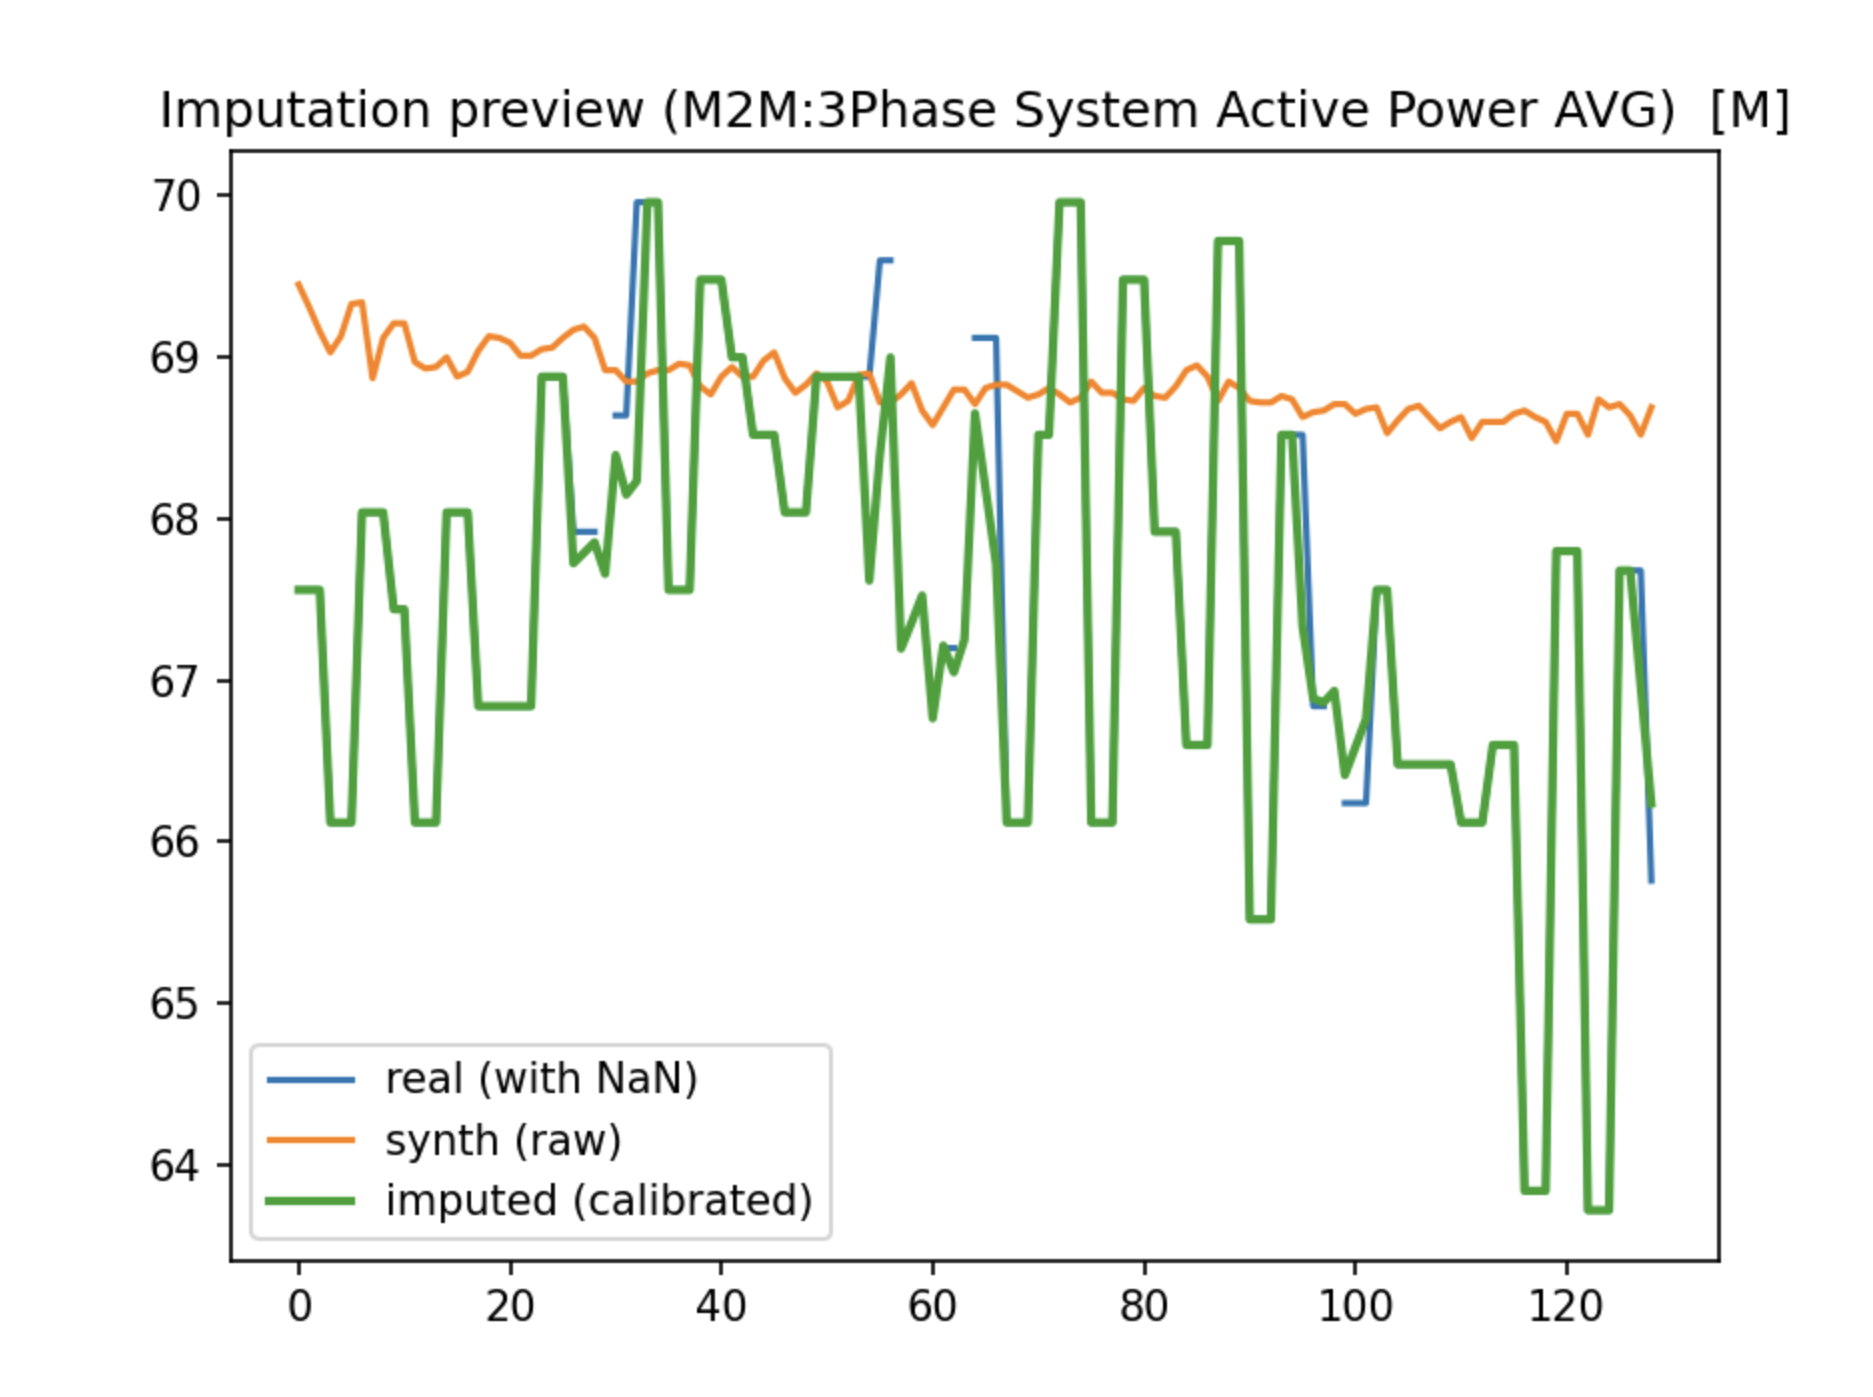
\includegraphics[width=0.60\textwidth]{images/Screenshot 2025-10-05 at 18.51.15}
\caption{Imputation on \emph{M2M}: the series with NaN is shown in blue, the synthetic trace in orange, and the calibrated local reconstruction in green.}
\label{fig:m2m_imputation}
\end{figure}

\begin{figure}[H]
\centering
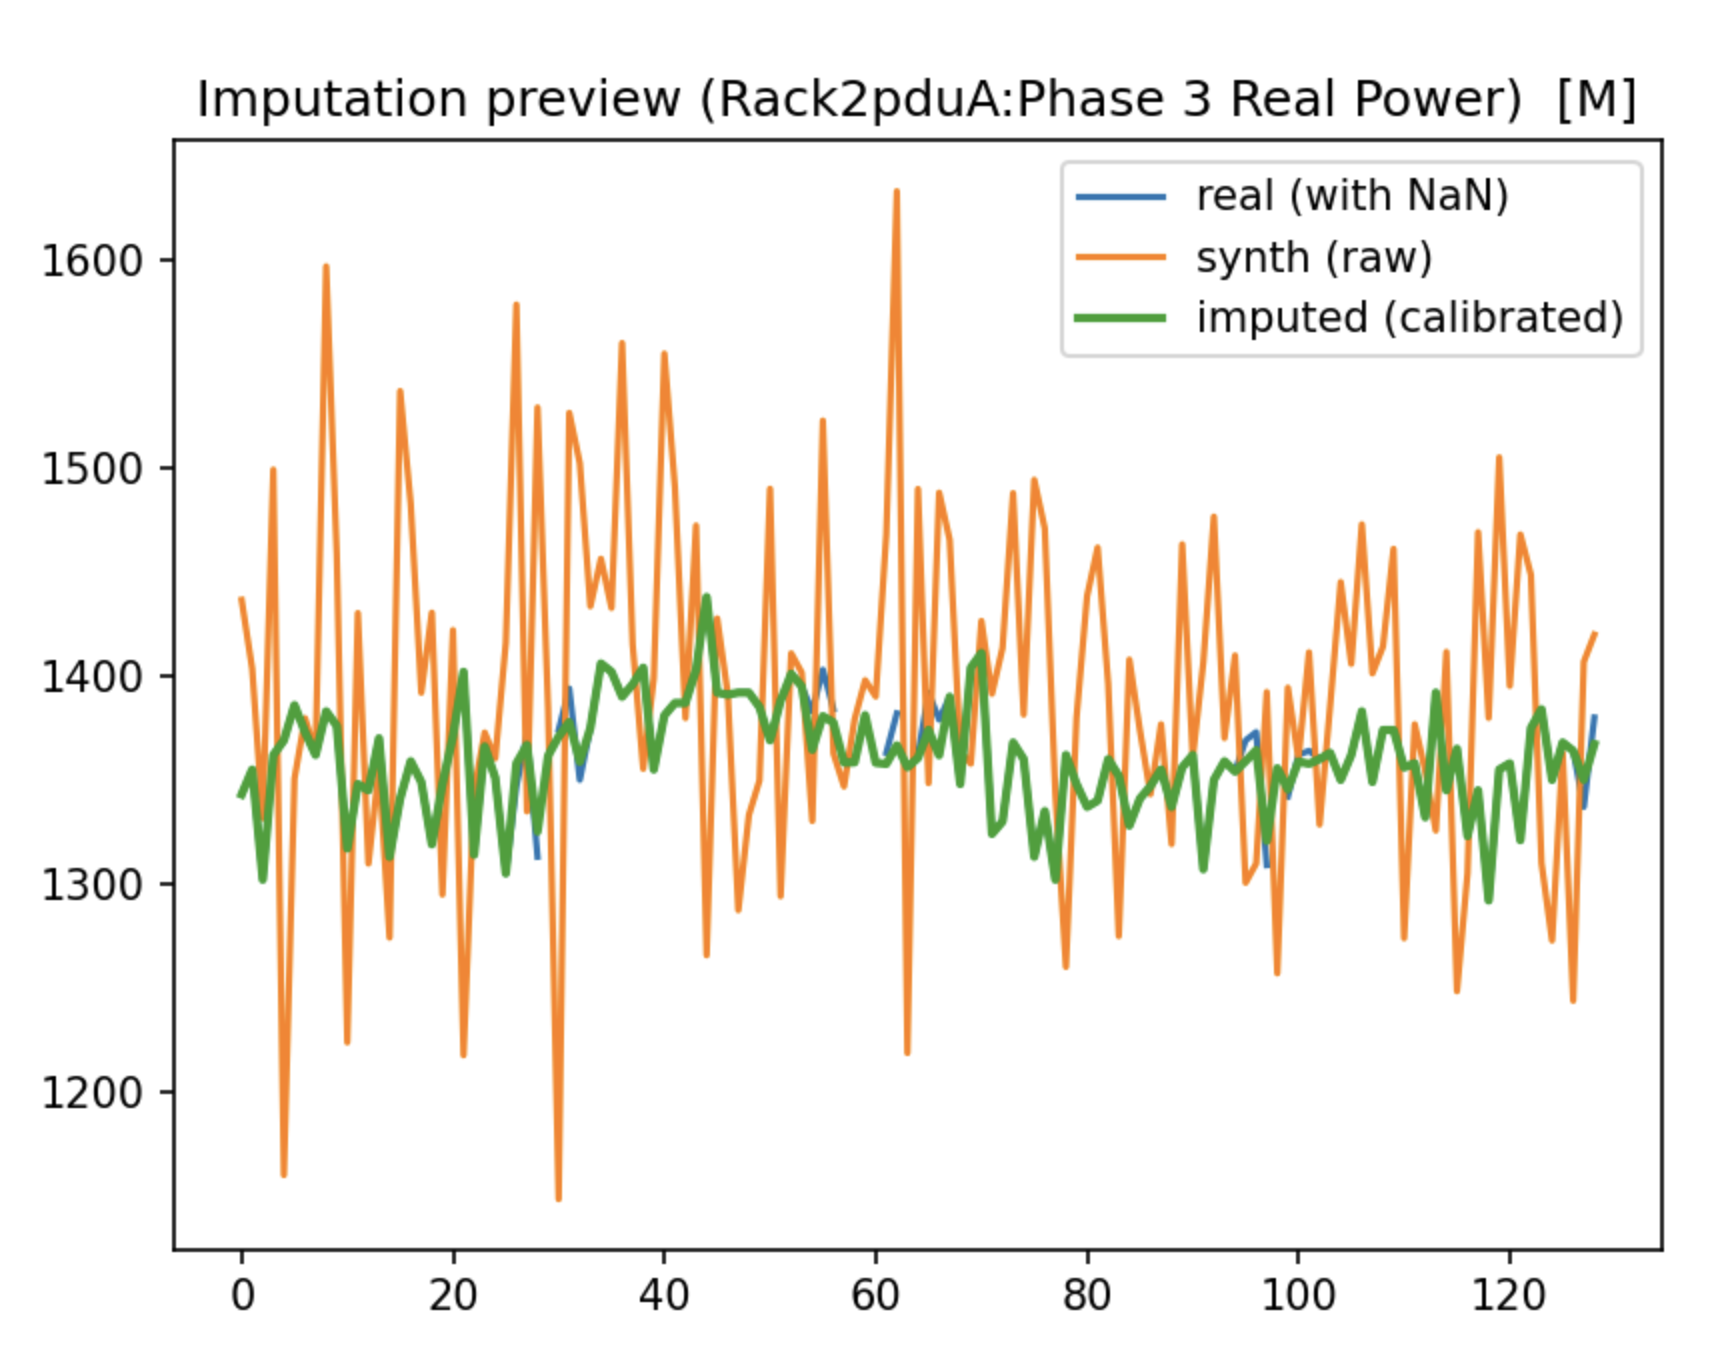
\includegraphics[width=0.60\textwidth]{images/Screenshot 2025-10-05 at 18.53.03}
\caption{Imputation on \emph{Rack2pduA}: attenuation of impulsive noise and preservation of the average trend.}
\label{fig:rack2pdua_imputation}
\end{figure}

\paragraph{Discussion.}
The results confirm that the imputation phase managed by \emph{WaveStitch} is effective in regular signals and remains surprisingly stable even in noisy contexts~\cite{che2018recurrent,luo2018multivariate}.  
The combination of \textbf{affine calibration} (to correct offset and scale differences), \textbf{quantile clipping} (to contain anomalous peaks), and the three generation masks (\emph{F, C, M}) allows the model to adapt to different reconstruction conditions.  
Overall, I observed a good balance between pointwise fidelity and statistical consistency of the filling, in line with the performance reported by the authors of \emph{WaveStitch} and consistent with the goal of generating reliable data even in the presence of real gaps or discontinuities.
% ----------------------------------------------------

\section{Structural Fidelity: ACD and xCorrDiff}

To go beyond point error-based evaluation, I wanted to investigate the \textbf{structural fidelity} of the synthetic series compared to the real ones.  
While MAE and RMSE measure numerical accuracy, these new metrics aim to understand whether the model is able to preserve the shape, temporal memory, and internal dependencies of multivariate signals.  
To this end, I adopted two complementary indicators also introduced by the authors of \emph{WaveStitch}:

\begin{itemize}
  \item \textbf{ACD} (\emph{Autocorrelation Difference}) — the absolute mean difference between the autocorrelation functions (ACF) of the real and synthetic series, calculated over lags $1,\dots,\tau_{\max}$;
  \item \textbf{xCorrDiff} — the average absolute difference between the correlation matrices of the real and synthetic multivariate data, limited to the upper triangle.
\end{itemize}

These two indicators allowed me to quantify more comprehensively the statistical plausibility of the generations, evaluating both \emph{intra-channel memory} (ACD) and \emph{inter-channel relationships} (xCorrDiff) — fundamental aspects for verifying the model’s dynamic consistency~\cite{hastie2009elements,box2015time,shumway2017time,wang2013experimental}.

\paragraph{Method.}
For each dataset $D \in \{\texttt{M2M}, \texttt{Rack2pduA}, \texttt{Rack3pduA}, \texttt{Rack5pduA}\}$ and for each conditioning mask $\texttt{F}/\texttt{C}/\texttt{M}$, I followed the procedure below:
\begin{enumerate}
  \item aligned the files \texttt{real.csv} and \texttt{synth*.csv} in time;
  \item selected only the common numerical columns;
  \item standardized each column using z-score normalization~\cite{bishop2006pattern,hastie2009elements};
  \item computed the autocorrelation functions up to $\tau_{\max}{=}50$ and their mean difference (\texttt{ACD\_mean});
  \item computed the correlation matrices and their mean difference on the upper triangle (\texttt{xCorrDiff\_mean}).
\end{enumerate}
For longer datasets, I performed the evaluations on the tail (last $N{=}5000$ samples), in order to maintain sensitivity to medium-term dependencies while reducing computational costs~\cite{hyndman2018forecasting}.

\begin{listing}[H]
\begin{minted}[fontsize=\footnotesize,breaklines,linenos,frame=lines,bgcolor=lightgray!10]{python}
import numpy as np
import pandas as pd

def acf_1d(x, max_lag=50):
    x = np.asarray(x, float) - np.nanmean(x)
    var = np.nanvar(x)
    if var <= 1e-12: return np.full(max_lag, np.nan)
    return np.array([np.nanmean(x[:-tau]*x[tau:])/var for tau in range(1, max_lag+1)])

def acd_mean_per_feature(R: pd.DataFrame, S: pd.DataFrame, max_lag=50):
    rows = []
    for c in R.columns:
        d = np.abs(acf_1d(R[c], max_lag) - acf_1d(S[c], max_lag))
        rows.append(dict(column=c, ACD_mean=np.nanmean(d)))
    df = pd.DataFrame(rows)
    return df, float(df["ACD_mean"].mean()) if not df.empty else np.nan

def xcorrdiff_mean(R: pd.DataFrame, S: pd.DataFrame):
    if R.shape[1] <= 1: return np.nan
    C_r, C_s = R.corr(), S.corr()
    iu = np.triu_indices(C_r.shape[0], k=1)
    return float(np.nanmean(np.abs(C_r.to_numpy()[iu] - C_s.to_numpy()[iu])))
\end{minted}
\caption{Implementation of ACF, ACD\_mean, and xCorrDiff\_mean.}
\end{listing}

\paragraph{Results.}
I am pleased to report that I obtained results consistent with the previous analyses.  
In more regular datasets such as \texttt{M2M}, the values of \textbf{ACD\_mean} and \textbf{xCorrDiff\_mean} are very low, indicating that the autocorrelative structures and inter-variable relationships are maintained extremely faithfully~\cite{box2015time,shumway2017time}.  
Conversely, in the noisier and more discontinuous rack datasets, these differences increase — a predictable behavior consistent with the intrinsic variability of loads and the lower statistical redundancy of local signals~\cite{wang2013experimental}.

\begin{table}[H]
\centering
\caption{Structural fidelity between real and synthetic series.}
\vspace{1mm}
{\small
\begin{tabular}{| l | c | c | c | c |}
\hline
\rowcolor[HTML]{F87C58}
\textbf{Dataset} & \textbf{Mask} & \textbf{n\_features} & \textbf{ACD\_mean} & \textbf{xCorrDiff\_mean} \\
\hline
\rowcolor[HTML]{FDE5DC}
M2M       & F/C/M & 9  & 0.130 & 0.358 \\ \hline
\rowcolor[HTML]{FFF4EE}
Rack2pduA & F/C/M & 16 & 0.699 & 0.491 \\ \hline
\end{tabular}
}
\label{tab:acd_xcorr_summary_2}
\end{table}

As an example, Table~\ref{tab:acd_per_feature_examples} shows the dispersion of ACD values for each channel: there is a high degree of homogeneity in the \emph{M2M} dataset and greater heterogeneity in individual racks, where local noise affects the stability of temporal patterns.

\begin{table}[H]
\centering
\caption{Example of per-feature ACD.}
\vspace{1mm}
{\small
\begin{tabular}{| l | l | c |}
\hline
\rowcolor[HTML]{F87C58}
\textbf{Dataset (mask)} & \textbf{Column} & \textbf{ACD\_mean} \\
\hline
\rowcolor[HTML]{FDE5DC}
M2M (F) & 3Phase System Active Energy & 0.102 \\ \hline
\rowcolor[HTML]{FFF4EE}
M2M (F) & 3Phase System Active Power AVG & 0.141 \\ \hline
\rowcolor[HTML]{FDE5DC}
Rack2pduA (F) & Phase 2 Energy & 0.984 \\ \hline
\rowcolor[HTML]{FFF4EE}
Rack2pduA (F) & Phase 3 Real Power & 0.486 \\ \hline
\end{tabular}
}
\label{tab:acd_per_feature_examples}
\end{table}

\paragraph{Interpretation.}
How can I interpret these results?  
A low \textbf{ACD\_mean} value indicates that the synthetic autocorrelations faithfully reproduce the periodicities and decays of the real series, preserving their dynamic memory.  
A low \textbf{xCorrDiff\_mean}, on the other hand, indicates that dependencies between channels — for example, between power, voltage, and current — are well preserved.  
Overall, these two indicators are the ideal complement to the numerical metrics, allowing me to evaluate the model not only in terms of accuracy but also in terms of internal consistency.

\subsection{Implications and Final Thoughts}
From this analysis, two key considerations emerge:

\begin{enumerate}
  \item \textbf{Role of structural metrics.}  
  I was able to verify that, in the presence of noisy signals, a low MAE does not necessarily guarantee dynamic fidelity.  
  To fill this gap, I complemented traditional metrics with the \emph{ACD} and \emph{xCorrDiff} indices, which also guided my preprocessing choices (clipping and cyclic normalization) and training regularization (e.g., \texttt{--stitch\_loss} and \texttt{--lambda\_corr}).  
  These metrics proved essential in identifying areas where the model tended to lose structural consistency.

  \item \textbf{Application reliability.}  
  On the \emph{M2M} dataset, the combination of \emph{stitching} and correlation regularization makes \emph{WaveStitch} particularly well suited for \emph{stress testing}, \emph{data augmentation}, and predictive simulations.  
  In the more irregular \emph{Rack*} datasets, I found it especially useful for \emph{imputation} and \emph{scenario design} tasks, where the model’s ability to maintain global consistency even under local variability represents a tangible advantage.  
  Nevertheless, structural adherence should be interpreted with caution in highly variable regions, where noise may mask part of the underlying physical relationships.
\end{enumerate}
